\documentclass{article}


\usepackage{arxiv}

\usepackage[utf8]{inputenc} % allow utf-8 input
\usepackage[T1]{fontenc}    % use 8-bit T1 fonts
\usepackage{hyperref}       % hyperlinks
\usepackage{url}            % simple URL typesetting
\usepackage{booktabs}       % professional-quality tables
\usepackage{amsfonts}       % blackboard math symbols
\usepackage{nicefrac}       % compact symbols for 1/2, etc.
\usepackage{microtype}      % microtypography
\usepackage{lipsum}
\usepackage{tikz}
\usepackage{dsfont}
\usepackage{amsmath}
\usepackage{array}
\usepackage{todonotes}
\usepackage{float}
\usepackage{rotating}
\usepackage[toc,page]{appendix} %appendix
\usepackage[sort&compress,square,comma,authoryear]{natbib}

\definecolor{maroon}{RGB}{176, 48, 96}
\definecolor{orange2}{RGB}{238, 118, 0}
\newcommand{\colindic}[1]{\textcolor{maroon}{#1}}
\newcommand{\colsurvey}[1]{\textcolor{orange2}{#1}}


\title{Early transmission pattern of Wuhan 2019-nCoV}


\author{
   Julien Riou \\
  Institute of Social and Preventive Medicine\\
  University of Bern\\
  Bern, Switzerland \\
  \texttt{julien.riou@ispm.unibe.ch} \\
  \And
Christian L.~Althaus \\
Institute of Social and Preventive Medicine\\
University of Bern\\
Bern, Switzerland \\
\texttt{christian.althaus@alumni.ethz.ch}
}



\begin{document}
\maketitle

\begin{abstract}
On December 31, 2019, the World Health Organization was notified about a cluster of pneumonia of unknown aetiology in the city of Wuhan, China. Chinese authorities later identified a new coronavirus (2019-nCoV) as the causative agent of the outbreak. As of January 23, 2020, 650 cases have been confirmed in China and several other countries. Understanding the transmission characteristics and the potential for sustained human-to-human transmission of 2019-nCoV is critically important for coordinating current screening and containment strategies, and determining whether the outbreak constitutes a public health emergency of international concern (PHEIC). We performed stochastic simulations of early outbreak trajectories that are consistent with the epidemiological findings to date. We found the basic reproduction number, $R_0$, to be around 2.2 (90\% high density interval 1.4--3.8), indicating the potential for sustained human-to-human transmission. Transmission characteristics appear to be of a similar magnitude to severe acute respiratory syndrome-related coronavirus (SARS-CoV) and the 1918 pandemic influenza. These findings underline the importance of heightened screening, surveillance and control efforts, particularly at airports and other travel hubs, in order to prevent further international spread of 2019-nCoV.
\end{abstract}

\section{Introduction}

\citet{Shi:2020}

- Info about outbreak
- Why it is important to understand transmission characteristics, and why we want to know $k$ and superspreading (limitation of study by Leung).

We used stochastic simulations in order to identify the likely transmission characteristics that have results in the early outbreak trajectory as reported to date.

\section{Methods}
We performed stochastic simulations of the first few generations of human-to-human transmission of 2019-nCoV. 
Simulations were initialized with one index case.
For each primary case, we generated secondary cases according to a negative-binomial offspring distribution with mean $R_0$ and dispersion $k$.\citep{Lloyd-Smith:2005,Althaus:2015b}
The dispersion parameter $k$ can be interpreted as a measure of the probability of superspreading events (the lower the value of $k$, the higher the probability of superspreading).
The generation time interval $D$ was assumed to be gamma-distributed with a shape parameter of 2, and a mean that varied between 7 and 14 days.
We explored a wide range of parameter combinations (Table \ref{fig:tab1}) and ran 1,000 stochastic simulations for each individual combination. 
This corresponds to a total of 3.52 million one-index-case simulations that were run on UBELIX (\url{http://www.id.unibe.ch/hpc}), the high performance computing cluster at the University of Bern. 

In a second step, we accounted for the uncertainty regarding the number of index cases $n$ and the date $T$ of the initial zoonotic animal-to-human transmissions at the wet market in Wuhan. 
An epidemic with several index cases can be considered as the sum of several independent epidemics with one index case each.
We sampled (with replacement) $n$ of the one-index-case epidemics, sampled a date of onset for each index case, and summed the epidemic curves together.
The sampling of the date of onset was done uniformly from a two-week interval around November 27, 2019, in coherence with early phylogenetic analyses of 11 2019-nCoV genomes.\cite{Rambaut:2020}
This step was repeated 10 times for each combination of $R_0$ (22 points), $k$ (20 points), $D$ (8 points) and $n$ (6 points) for a total of 211,200 full epidemics simulated.
Finally, we calculated the proportion of stochastic simulations that reached a total number of infected cases within the interval [1000, 9700] by January 18, 2020, as estimated by Imai and colleagues.\citep{Imai:2020}
In a process related to approximated Bayesian computation (ABC), the parameter value combinations that led to simulations within that interval were treated as approximations to the posterior distributions of the parameters with uniform prior distributions.
Model simulations and analyses were performed in the R software for statistical computing.\citep{R:2018} 
Code files are available on \url{https://github.com/jriou/wcov}.

\begin{table}
	\centering
	\caption{Parameter ranges for stochastic simulations of outbreak trajectories.}
	\label{fig:tab1}
\begin{tabular}{llll}
	\hline
	Parameter & Description & Range   \\
	\hline 
	$R_0$& Basic reproduction number  &[0.8 -- 5.0] \\ 
	$k$ & Dispersion parameter & [0.01 -- 10] \\
	$D$ & Generation time interval & [7 -- 14]  \\
	$n$ & Initial number of index cases & [1 -- 50]  \\
	$T$ & Date of zoonotic transmission & [20 Nov 2019 -- 4 Dec 2019] \\
	
	\hline 
\end{tabular} 
\end{table}

\section{Results}
In order to reach between 1000 and 9,700 infected cases by January 18, 2020, the early human-to-human transmission of 2019-nCoV must be either characterized by values of $R_0$ around around 2.2 (90\% high density interval 1.4--3.8) (figure \ref{fig:fig2}).
Observed data at this point is compatible with a large range of values for the dispersion parameter $k$. 
However, our simulations indicate that very low values of $k$, corresponding to a large probability of superspreading events, are less likely.
These estimates incorporate the uncertainty on the current total epidemic size (as of January 23, 2020) and on the date and scale of the initial zoonotic event (figure \ref{fig:fig3}).

Comparison with other emerging viruses allows to put in perspective the low amount of information available regarding the transmission patterns of 2019-nCoV.
Our estimates of $R_0$ and $k$ are more similar to previous estimates focusing on early human-to-human transmission of SARS-CoV in Beijing and Singapore\cite{Lloyd-Smith:2005} than of MERS-CoV\cite{Kucharski:2015b} (figure \ref{fig:fig1}).
These estimates are also in line with those of 1918 Influenza.\cite{Fraser:2011}


%([2, 5]) and low values of $k$ (< 1). The latter scenario is similar to what has been estimated for SARS-CoV and indicates the considerable potential for superspreading of 2019-nCoV.

\begin{figure}[h]
	\centering
	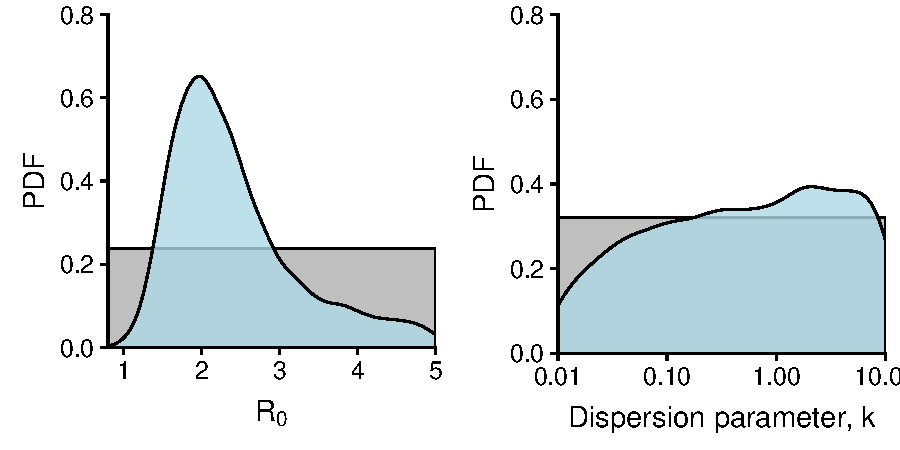
\includegraphics[width=.6\linewidth]{../figure/fig2.pdf}
	\caption{Values of the basic reproduction number $R_0$ and of the dispersion parameter $k$ most compatible with epidemic data available on 2019-nCoV as of January 23, 2020.}
	\label{fig:fig2}
\end{figure}


\begin{figure}[h]
	\centering
	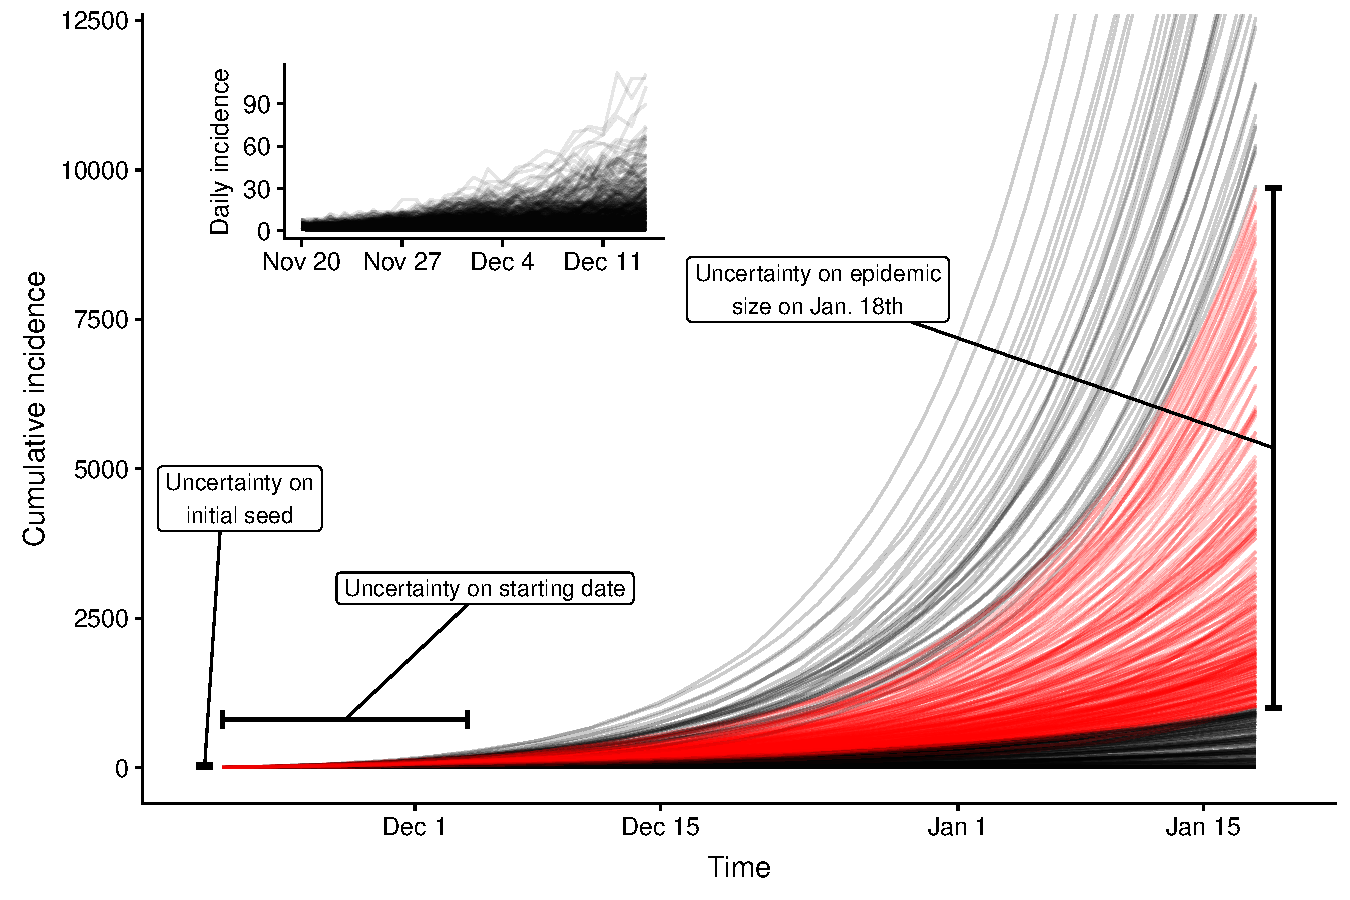
\includegraphics[width=.9\linewidth]{../figure/fig3b.pdf}
	\caption{Illustration of the simulation strategy. The lines represent the cumulative incidence of 100 simulations with $R_0=1.8$ and $k=1.62$ that led to 62.5\%. Trajectories in red are deemed compatible with the estimated total size of the epidemic on January 18, 2020 (the last available estimate as of January 23, 2020).}
	\label{fig:fig3}
\end{figure}


\begin{figure}[h]
	\centering
	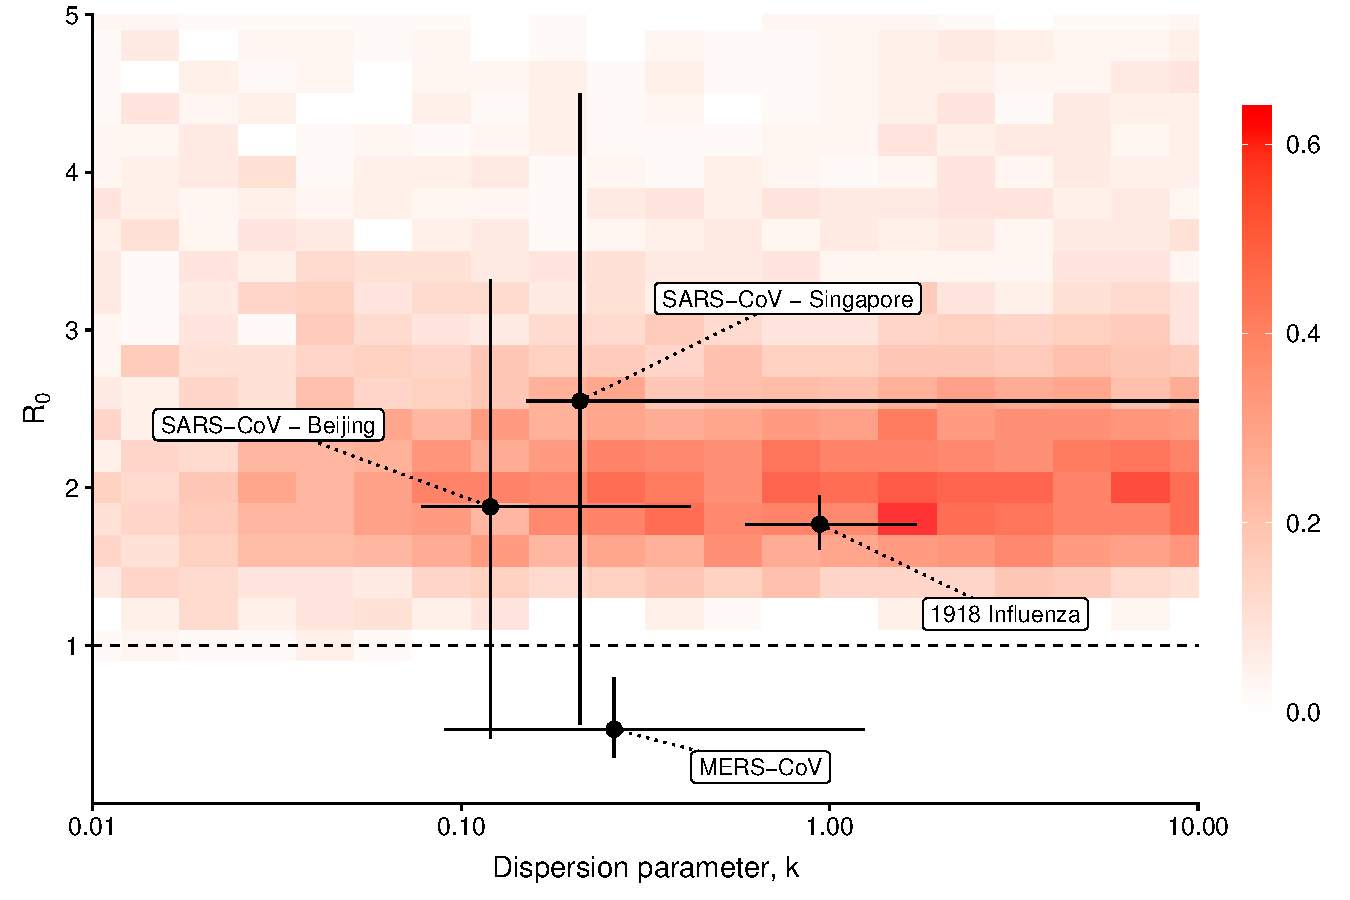
\includegraphics[width=.9\linewidth]{../figure/fig1.pdf}
	\caption{ Comparison of the estimates of $R_0$ and $k$ for 2019-nCoV with corresponding parameters for the early human-to-human transmission of SARS-CoV in Singapore and Beijing, and of 1918-Influenza.\cite{Lloyd-Smith:2005,Fraser:2011,Kucharski:2015b}
	}
	\label{fig:fig1}
\end{figure}


\section{Discussion}

Concerns are spreading regarding the emergent 2019-nCoV in Wuhan, China.
As WHO is discussing about PHIEC but lacks information about the patterns of transmission of the disease
This analysis focuses on the few data points available to


- List primary finding
- Why it is important to consider superspreading and negative-binomial offspring distributions
- Still limited data (range depends on estimate as well)
- SARS-like transmission underlines potential for pandemic
- Screening and international efforts crucial at this stage


\section{Acknowledgements}
JR is funded by the Swiss National Science Foundation (grant 174281).
\section{Conflict of interest}
None declared.

\section{Authors' contributions}

JR and CLA designed the study, JR performed model simulations, JR and CLA analyzed and interpreted the results and wrote the manuscript.

\bibliography{ncov.bib}
\bibliographystyle{unsrt}  
\end{document}
